%
% File: chap01.tex
% Author: Victor F. Brena-Medina
% Description: Introduction chapter where the biology goes.
%
\let\textcircled=\pgftextcircled
\chapter{Architecture}
\label{chap3}
\initial{T}his project focuses on two-person human-human interaction recognition and detection in videos. Almost all of the few previous works \cite{patron2010} \cite{narayan2014} \cite{choi2012} in two-person human-human interaction recognition  adopt hand-crafted feature descriptors. For example, Narayan et al. \cite{narayan2014} combine improved trajectory features and foreground motion map features to present interaction features while Patron-Perez et al. \cite{patron2010} and Choi et al. \cite{choi2012} use a hierarchical model to present interaction features. In the hierarchical model,  each individual is tracked throughout the videos, and the atomic activity for each individual and their relative position and orientations are computed firstly then the collective interaction is represented. Our work adopts the hierarchical model similar to \cite{patron2010} but we replace the hand-crafted feature descriptors with deep learning feature descriptors since deep learning based methods \cite{Ji2013} \cite{Tran2015} \cite{simonyan2014} \cite{Ng2015} have already achieve better performance in closely related domain, single person action recognitions in videos, than hand-crafted feature descriptors\cite{grepory2010} \cite{alex2008} \cite{paul2007} \cite{wang2012} \cite{wang2013}. 
    
\section{Overall Framework}
\label{3_1}
Since the deep network has a very strong ability for feature learning and description, the most direct way is just feeding the whole video into a deep network and train it. Such a network can achieve decent performance if the training datasets are proper and rich enough. But for our project, two-person interaction recognition and detection, we only have three small scale two-person interaction datasets: \textbf{UT-Interaction} \cite{ut2010}, \textbf{ShakeFive2} \cite{shakefive2} and \textbf{MMI} \cite{m2i_tju}  with very limited training samples. It is insufficient to train a deep learning network to achieve a nice performance on these datasets.  But fortunately, we do have many large scale single person action datasets, like \textbf{UCF-101} \cite{ucf101},\textbf{Sports-1M}, \textbf{Activity-Net200} \cite{activitynet200}, etc. We can use those large scale dataset to pre-train our deep learning network and finetune it with the target interaction dataset.
\par 
Due to lack of sufficient proper two-person interaction datasets to just train a deep network, we adopt the hierarchical model similar with \cite{choi2012} and  \cite{patron2010} which learn atomic action features for each individual in the video and combine these features to represent the collective interaction features. Different with \cite{choi2012} and \cite{patron2010} that use hand-crafted features, such as HOG and BoV, we use deep learning networks as the feature descriptors.
\par    
In our architecture, we first apply person detection to localize the positions of each person in the videos and then crop the video into  two-video volumes, each containing one person's activity. Then we design an atomic action spatial-temporal feature descriptor for each person. Since there are lots of large scale single person action datasets available, we can pre-train the atomic action feature descriptors with those datasets and finetune the parameters on interaction datasets.
\par 
One drawback of this hierarchical model is ignoring the important relative information between the two-person, such as relative position and orientation, etc. So, we introduce another overall feature descriptor to learn those relative information which can be trained directly from our target dataset \textbf{UT-Interaction}. 
\par 
 The fusion of all learned features are fed to a SVM classifier. The overall framework is illustrated in Figure \ref{fig:overall_arch}.
 
 
 \begin{figure}
 	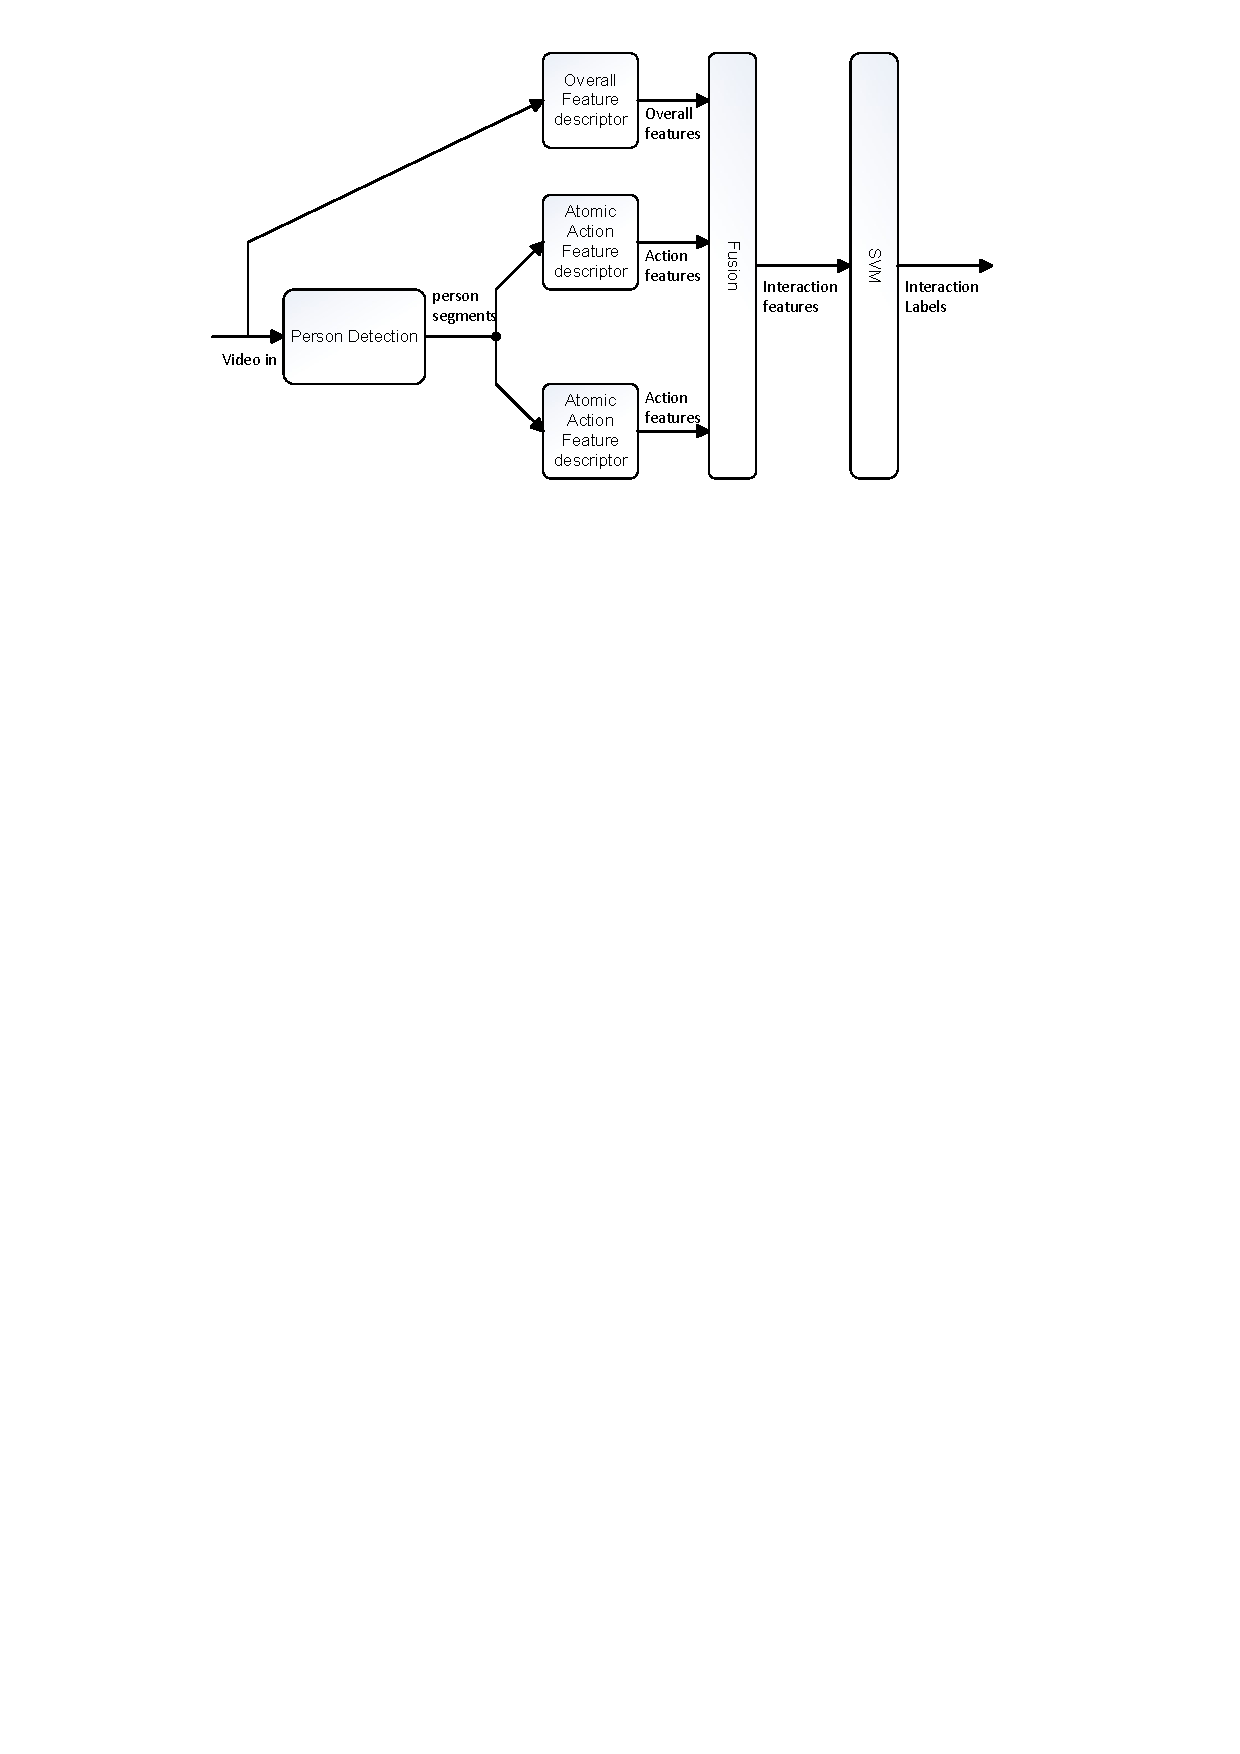
\includegraphics[trim=2cm 21.5cm 0cm 1cm]{fig01/architecture.pdf}
 	\caption{Overall framework. }
 	\label{fig:overall_arch}
 \end{figure}

\section{Person Detection}
\label{3_2}
In this project, we have three interaction video dataset available, \textbf{UT-Interaction}, \textbf{ShakeFive2} and \textbf{MMI} respectively. And joint information is provided for \textbf{ShakeFive2} and \textbf{MMI}. In the dataset \textbf{UT-Interaction}, all videos are filmed in static cameras with simple background and without much people occlusion. So, We use classical HOG plus SVM framework to construct person detector \cite{inria_person}. The structure of person detection is illustrated in Figure \ref{fig:person_detection}.  
\par 
The Person Detection module will detect the location of people in each frame and track two people throughout a video. The crops for each person will be resized to the same size and construct two video volumes.  
        
\begin{figure}
	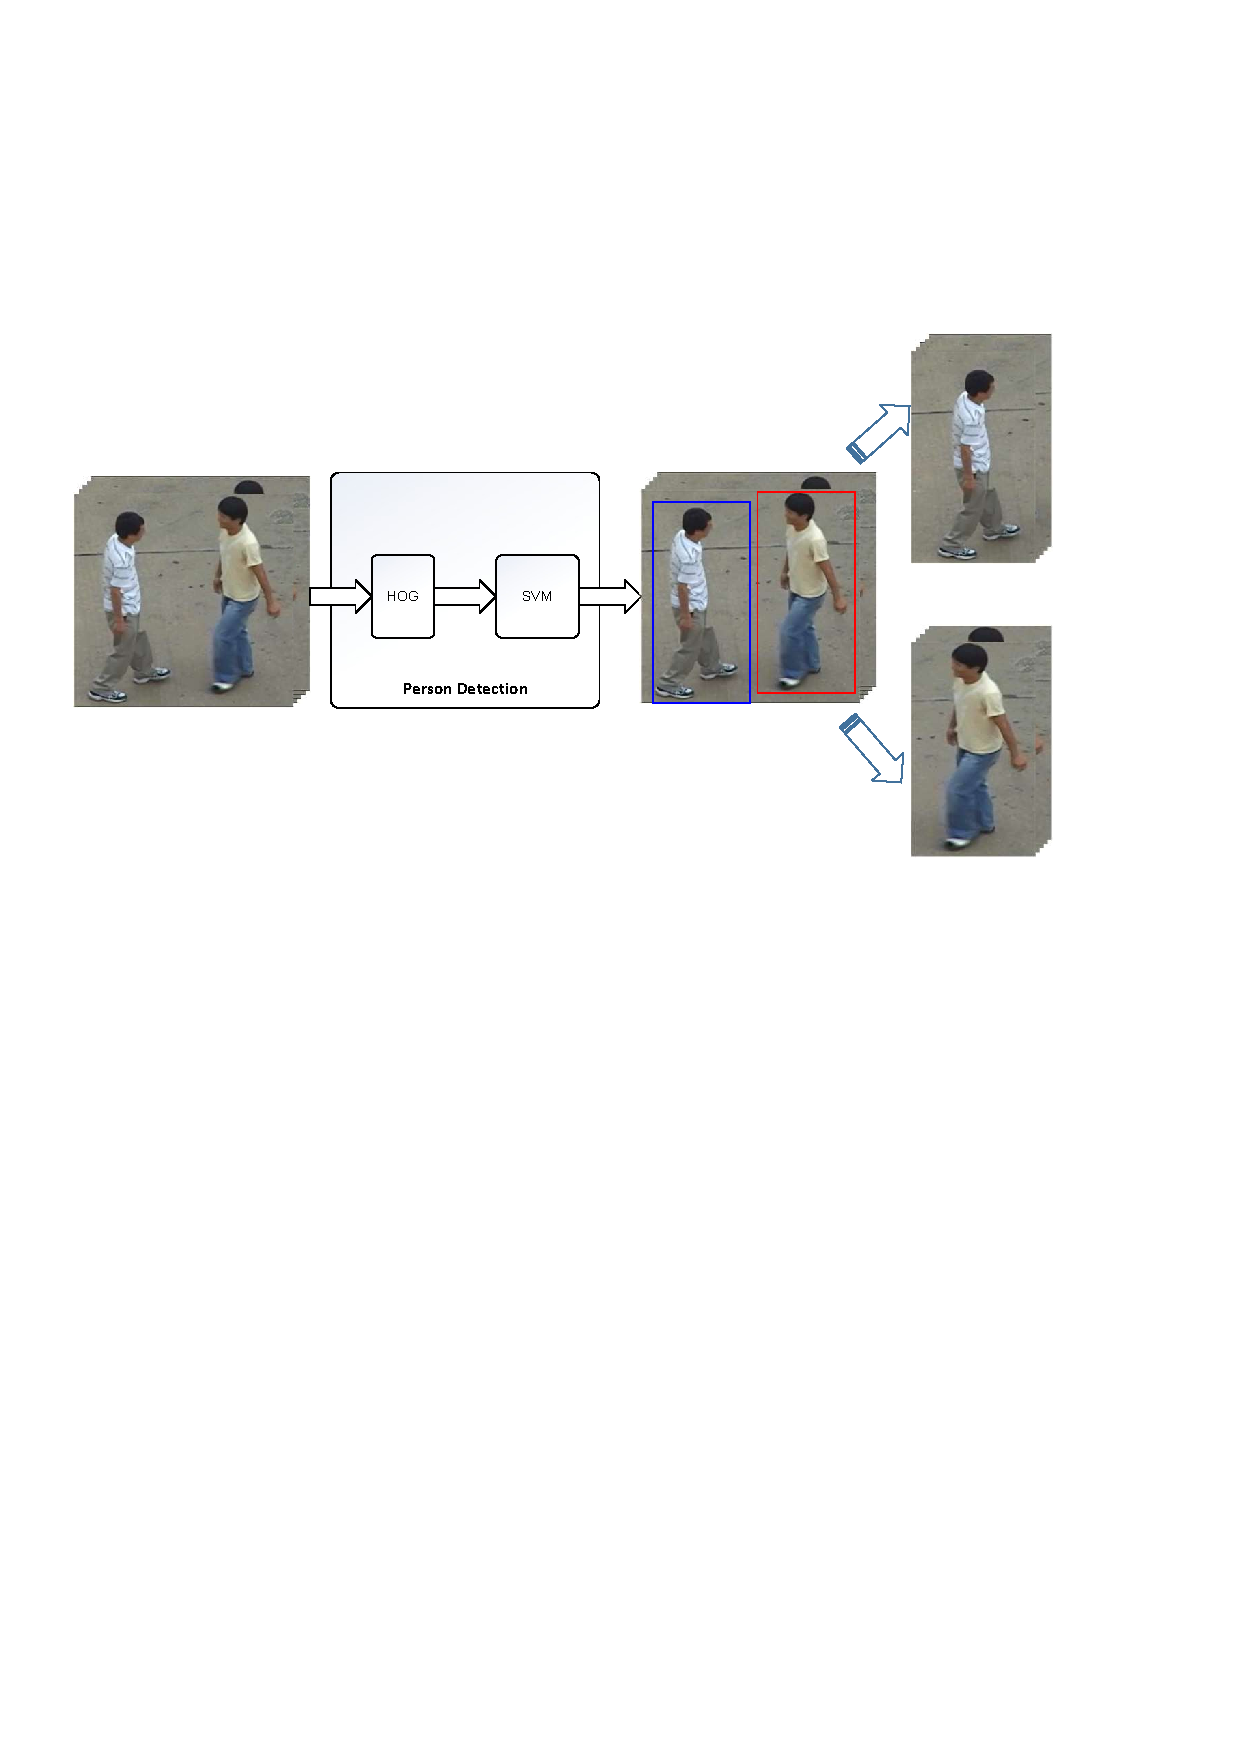
\includegraphics[trim=2cm 15cm 0cm 5cm]{fig01/person_detection.pdf}
	\caption{Illustration of Person detection  }
	\label{fig:person_detection}
\end{figure}

\section{Feature Descriptors}
\label{3_3}
We have two-level hierarchical feature descriptors in the project: an overall feature descriptor which learns the global features such as the relative position and orientation between two-person and two atomic feature descriptors which learn the local atomic action features for each person. The overall feature descriptor and atomic action feature descriptors share similar network frameworks. We use different parameters between overall feature descriptor and atomic feature descriptor while sharing the parameters between two atomic action feature descriptors. That is, we only train one atomic action feature descriptor for one person and totally duplicate it for another person.  
\par 
Since temporal information is a very important factor for video analysis, we adopt two different types of spatial-temporal feature descriptor to present the overall and atomic action features: 3D Convolutional Network(3D-ConvNet)\cite{Tran2015} and Two-Stream Convolutional Network(Two-Stream ConvNet) \cite{simonyan2014} respectively. Because above two type of spatial-temporal feature descriptor have already achieved very nice performance in video action recognition tasks. And they present the spatial-temporal features from different views: three dimensional(x,y,time) convolution for 3D-ConvNet and two dimensional(x,y) convolution on still frames plus multiple frame motion optical-flow convolution for Two-Stream ConvNet. We will compare their performance in interaction recognition and detection tasks among these two methods and even combine output features of these two methods together to see whether we can get better performance. 
 
\subsection{3D-ConvNet}
\label{3_3_1}
3D ConvNet learns both spatial and temporal features at the same time by applying three-dimensional (x,y,time) convolution and pooling. We use the similar architecture as Tran et al.'s 3D-ConvNet\cite{Tran2015} as our 3D-ConvNet based feature descriptor. The architecture of 3D-ConvNet is illustrated in Figure \ref{fig:c3d}. 
\begin{figure}
	\includegraphics[trim=2cm 26cm 0cm 1cm]{fig01/3dConvNet.pdf}
	\caption{Overall Architecture of 3D-ConvNet. }
	\label{fig:c3d}
\end{figure}

\subsection{Two-Stream ConvNet}
\label{3_3_2}
Different with a 3D-ConvNet learns spatiotemporal features in a single network, the two-stream ConvNet learns spatial features and temporal features in two separate 2D convolutional networks. The spatial stream network learns spatial features from single input frame and the temporal stream network learn temporal features from multiple frames of optical flow which represents the motion information between the consecutive frames. We take a similar architecture as the work of Simonyan et al.\cite{simonyan2014} as our two-stream ConvNet. The spatial and temporal features fuse at the end of two ConvNet to represent the overall features of input videos. The overall architecture of two-stream ConvNet is illustrated in Figure \ref{fig:tsconvnet}.
\begin{figure}
	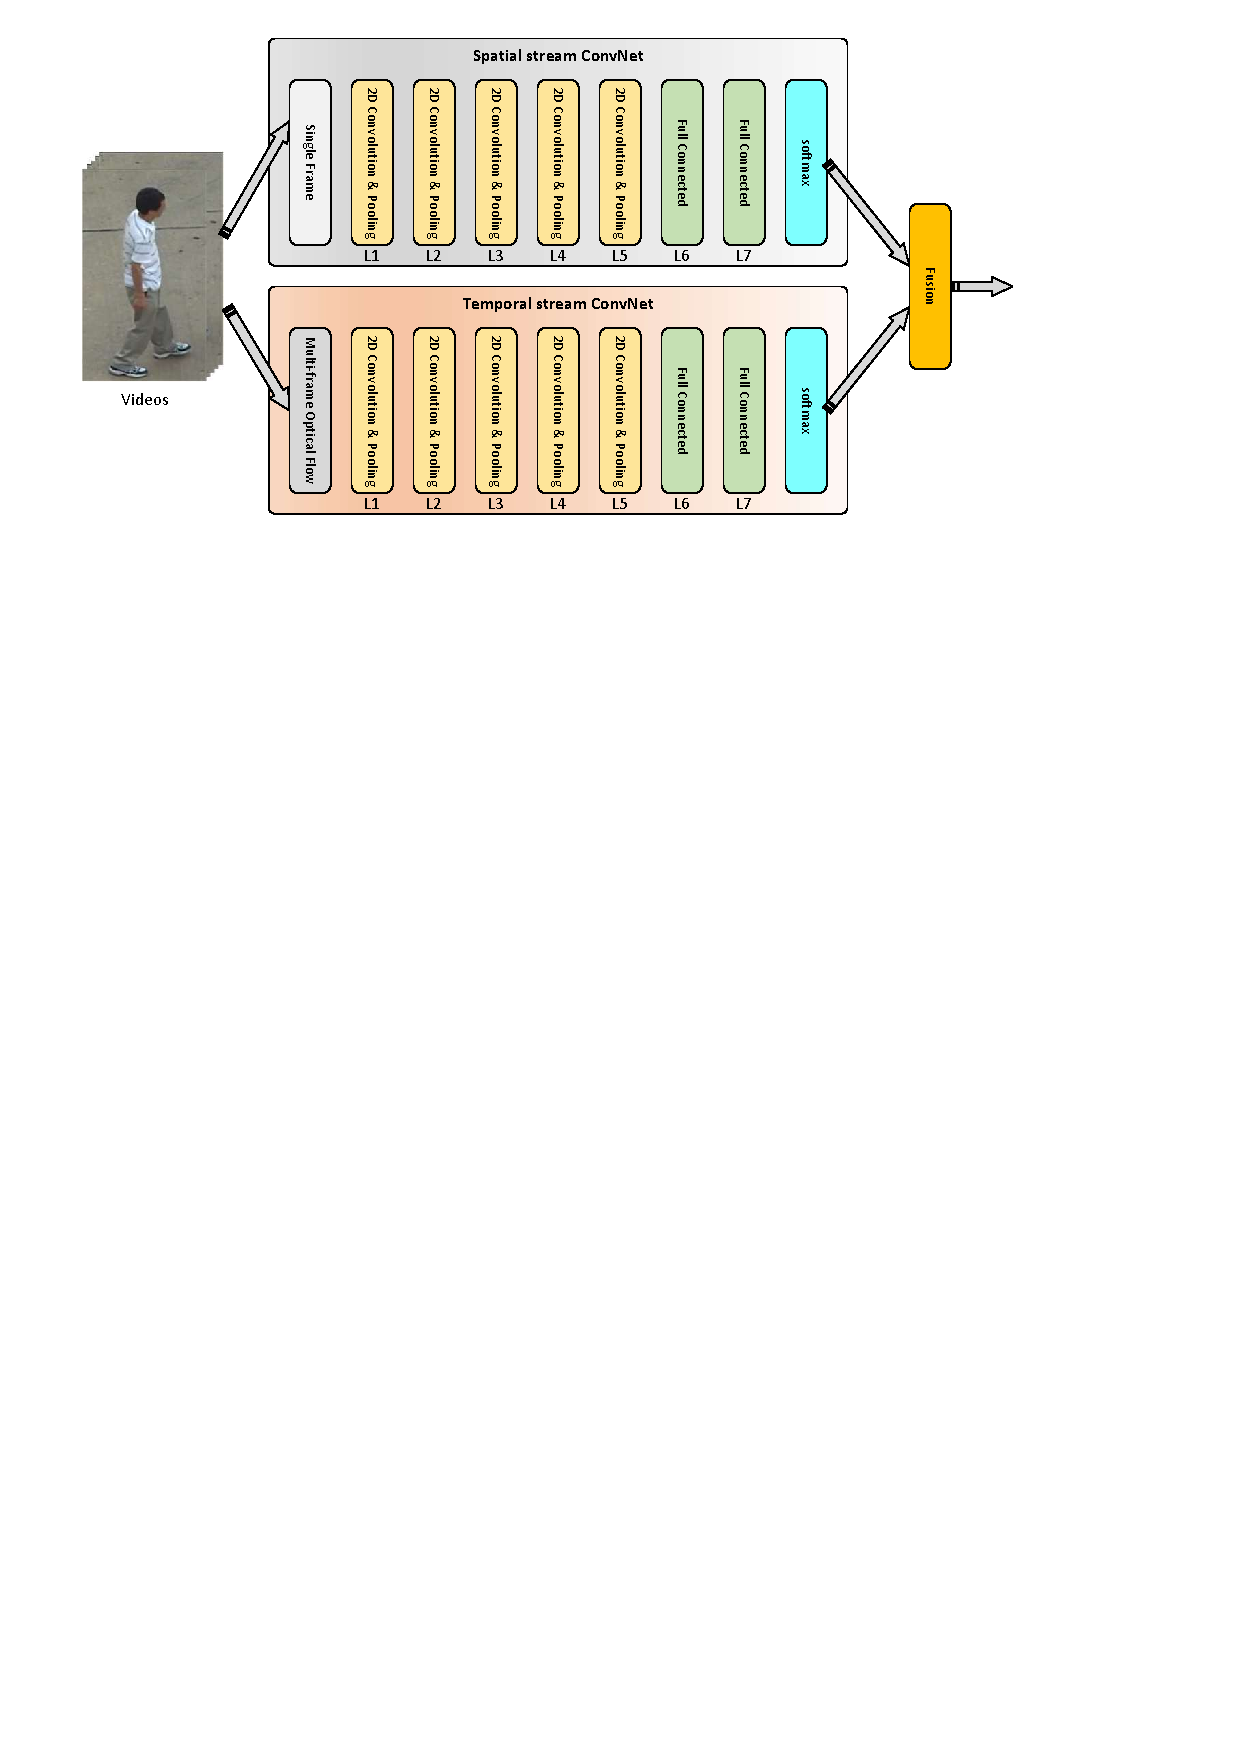
\includegraphics[trim=2cm 21cm 0cm 1cm]{fig01/TSConvNet.pdf}
	\caption{Overall Architecture of Two-Stream ConvNet. }
	\label{fig:tsconvnet}
\end{figure}

\section{Training}
\label{3_4}
Since the performance of a learning algorithm is highly dependent on the training datasets, it is important to select proper training datasets for each network and balance the performance and computational complexity at the same time.
  
\subsection{Train Person Detection Network}
We select \textbf{INRIA Person Dataset} \cite{inria_person} to train our person detection network. INRIA Person Dataset is one of the most used datasets for static people detection which provides original images and corresponding annotations. The training set contains 614 (2416 people) positive images and 1218 negative images. The testing set contains 288 (1126 people) positive images and 453 negative images. Only upright persons (with height larger than 100 pixels) are marked in each image. The sources of this dataset are mainly collected from GRAZ01 dataset, personal digital images, and Google images. Most of them have very high resolutions.

\subsection{Train 3D-ConvNet}
We adopt different training strategies between overall feature descriptor and atomic action feature descriptors. 
\par
Due to that the overall features descriptor learns to present interaction features and the target interaction video dataset \textbf{UT-Interaction} \cite{ut2010} is a small scale dataset, we will pre-train the overall feature descriptor on other interaction video datasets: \textbf{ShakeFive2} \cite{shakefive2} or \textbf{MMI} \cite{m2i_tju}, then fine-tune it on \textbf{UT-Interaction} dataset.
\par
For the atomic action feature descriptors, because we have large scale single person action datasets available and the complexity of 3D-ConvNet, we adopt the pre-training and fine-tune strategy to train this network. Large scale action video dataset \textbf{UCF-101} \cite{ucf101} or \textbf{Activity-Net200} \cite{activitynet200} will be used to pre-train the 3D-ConvNet.
\par 
In pre-training phase, we will feed the videos and labels of above two datasets to the 3D-ConvNet plus a softmax classifier. Then the 3D-ConvNet will learn the features from those videos and labels. 
\par 
In fine-tuning phase, we will feed videos and labels of \textbf{UT-Interaction} to the pre-trained network. All parameters of convolutional layers of pre-trained network remain and only parameters of fully connected layers will be fine-tuned. 

\subsection{Train The SVM Classifier}
All output features of overall feature descriptor \(fg\) and atomic action feature descriptors \(fa0\) and \(fa1\) are fused and fed to a one-vs-the-rest SVM classifier. The SVM classifier is trained with the target dataset \textbf{UT-Interaction}.

\section{Testing}
\label{3_5}
We use \textbf{UT-Interaction}\cite{ut2010} to evaluate our interaction recognition and detection network for both interaction classification and detection. \textbf{UT-Interaction} dataset has 120 segmented videos (two sets, 60 videos for each set) for classification task and 20 videos with spatial and temporal ground truth annotations for detection task.      
\par 
For test 'classification' task, the two sets of videos are evaluated separately. 10-fold leave-one-out cross validation is used to evaluate the classification accuracy. The performance is measured ten times and average accuracy is used as the overall accuracy. 
\par 
For the 'detection' task, the interaction detection is measured to be correct if and only if the network correctly annotates an occurring interaction's time interval and spatial bounding box. If the annotation overlaps the ground truth more than 50\% spatially and temporally, the detection is treated as a true positive. Otherwise, it is treated as a false positive.  

%=========================================================